% Dies ist Teil der Vorlesung Physik auf dem Computer, SS 2012,
% Axel Arnold, Universitaet Stuttgart.
% 
% Dieses Werk ist unter einer Creative Commons-Lizenz vom Typ
% Namensnennung-Weitergabe unter gleichen Bedingungen 3.0 Deutschland
% zugänglich. Um eine Kopie dieser Lizenz einzusehen, konsultieren Sie
% http://creativecommons.org/licenses/by-sa/3.0/de/ oder wenden Sie sich
% schriftlich an Creative Commons, 444 Castro Street, Suite 900, Mountain
% View, California, 94041, USA.

\chapter{Nichtlineare Gleichungssysteme}
\index{Gleichungssysteme>nichtlineare}
\index{Nullstellensuche}
\index{Fixpunktbestimmung}

Im zweiten Kapitel hatten wir uns mit der Lösung linearer
Gleichungssysteme beschäftigt, die ja eine wesentliche Grundlage der
numerischen Mathematik darstellen. Allerdings tauchen in der Praxis,
besonders in der Physik, leicht auch nichtlineare Gleichungssysteme
auf. In diesem Fall kann man meist keine allgemeine Aussage über
Existenz und Anzahl der Lösungen machen, und kann auch keine exakten
Verfahren zur Lösung angeben.

Nichtlineare Gleichungssysteme werden typischerweise in zwei Formen
betrachtet. Sei eine Funktion $f:\RR^n\to\RR^m$ gegeben. Dann suchen
wir die \emph{Nullstellen}
\begin{equation}
  \label{eq:nullstellen}
  x, \quad\text{so dass}\; f(x) = 0,
\end{equation}
also die Lösungen zur Gleichung $f(x) = 0$. Alternativ können wir für
eine Funktion $f:\RR^n\to\RR^n$ die \emph{Fixpunkte} suchen. Diese
sind
\begin{equation}
  \label{eq:fixpunkt}
  x, \quad\text{so dass}\; g(x) = x,
\end{equation}
also die Lösungen der Gleichung $g(x) = x$. Eine Fixpunktgleichung
lässt sich natürlich stets auch als Nullstellenproblem mit $f(x) =
g(x) - x$ formulieren; anders herum geht dies im allgemeinen nicht.

Die beiden Formulierungen unterscheiden sich allerdings im natürlichen
Lösungsansatz. Die Nullstellengleichung \eqref{eq:nullstellen} ähnelt
dem linearen Gleichungssystem \eqref{eq:lgs}. Das
\emph{Newtonverfahren} beruht auf einer lokalen Linearisierung und dem
Lösen dieses linearen Gleichungssystems. Die Fixpunktgleichung
hingegen legt nahe, den Fixpunkt durch \emph{sukzessive Substitution}
zu suchen: $x_0\to g(x_0)\to g(g(x_0))\to\ldots$.

\section{Sukzessive Substitution}
\index{sukzessive Substitution}
\index{Fixpunktbestimmung}

Eine Abbildung $g:M\to M$ mit $M\subset\RR^n$ heißt Lipschitz-stetig
(L-stetig), falls es ein $L\in\RR$ gibt, so dass
\begin{equation}
  \norm{g(x) - g(y)} \le L \norm{x - y}\quad\forall x,y\in M.
\end{equation}
Alle auf $M$ differenzierbaren Funktionen mit beschränkter Ableitung
sind L-stetig, wenn ihre Ableitung beschränkt ist. Die
Lipschitzkonstante ergibt sich aus dem Mittelwertsatz zu $L=\max_{x\in
  M}\norm{g'(x)}$.  Es gibt allerdings noch mehr L-stetige Funktionen,
zum Beispiel die in 0 nicht differenzierbare Betragsfunktion, die auf
ganz $\RR$ L-stetig mit $L = 1$ ist. Auf der anderen Seite ist
offenbar jede L-stetige Funktion auch stetig, d.h., die L-stetigen
Funktionen sind eine eigene Klasse zwischen den stetigen und
differenzierbaren Funktionen.

\index{Banachscher Fixpunktsatz} Hat eine Funktion $g:M\to M$ eine
Lipschitz-Konstante $L<1$, so heißt $g$ \emph{kontrahierend}, weil
zwei verschiedene Punkte durch die Abbildung stets näher aneinander
geschoben werden. Wir betrachten nun einen beliebigen Startpunkt
$x_0\in M$ und definieren damit die Folge der \emph{sukzessive Substitution}:
\begin{equation}
  x_{n} := g(x_{n-1}) \quad\text{für}\; n\ge 1.
\end{equation}
Dann gilt für alle $n,m\in\NN$ der \emph{Banachsche Fixpunktsatz}
\begin{align}
  \label{eq:banach}
  \norm{x_{n+m} - x_n} \,=\, &\norm{\sum_{k=0}^{m-1} x_{n+k+1} - x_{n+k}}
  \,\le\, \sum_{k=0}^{m-1} \norm{x_{n+k+1} - x_{n+k}}\nonumber\\
  \,=\, &\norm{g(g(...g(x_{n+1}))) - g(g(...g(x_{n})))}
  + \cdots\nonumber\\
  &+ \norm{g(g(x_{n+1})) - g(g(x_{n}))}
  + \norm{g(x_{n+1}) - g(x_{n})} + \norm{x_{n+1} - x_{n}}\nonumber\\
  \le\, &\sum_{k=0}^{m-1} L^k \norm{x_{n+1} - x_{n}}
  \,\le\, \frac{1}{1-L}\norm{x_{n+1} - x_{n}} \le
  \frac{L^n}{1-L}\norm{g(x_0) - x_0}.
\end{align}
Die sukzessive Substitution definiert also eine Cauchyfolge, die in
$M$ konvergiert, sofern $M$ abgeschlossen ist (z.B. $M=\RR^n$ oder $M$
Einheitskugel). Für den Grenzwert $\overline{x}$ dieser Folge gilt
\begin{equation}
  \overline{x} = \lim_{n\to\infty}x_{n+1} = \lim_{n\to\infty}g(x_{n})
  = g(\overline{x}),
\end{equation}
er ist also ein Fixpunkt.

Wir betrachten nun zwei Fixpunkte $\overline{x}$ und $\overline{y}$. Dann gilt
\begin{equation}
  \norm{\overline{x} - \overline{y}} = \norm{g(\overline{x}) -
    g(\overline{y})} \le L \norm{\overline{x} - \overline{y}} \implies
  \overline{x} = \overline{y}.
\end{equation}
Das bedeutet, dass es nur genau einen Fixpunkt $\overline{x}$ von $g$
in $M$ gibt, und dass die sukzessive Substitution für jeden Startwert
\emph{global} gegen $\overline{x}$ konvergiert. \eqref{eq:banach}
gibt auche eine \textit{a priori}-Abschätzung des Fehlers:
\begin{equation}
  \norm{\overline{x} - x_n} \le \frac{L^n}{1-L}\norm{g(x_0) - x_0}
\end{equation}
sowie eine Abschätzung der Konvergenzrate:
\begin{equation}
  \frac{\norm{x_{n+1} - \overline{x}}}{\norm{x_n - \overline{x}}}
  = \frac{\norm{G(x_n) - G(\overline{x})}}{\norm{x_n - \overline{x}}}
  \le L < 1.
\end{equation}
Die sukzessive Substitution konvergiert also linear.

Neben dieser globalen Konvergenzeigenschaft konvergiert die sukzessive
Substituion auch lokal: ist $g:\RR^n\to\RR^n$ eine differenzierbare
Funktion und hat einen Fixpunkt $\overline{x}$ mit $\norm{g'(x)} < 1$,
so gibt es eine Umgebung des Fixpunktes, in dem die sukzessive
Substitution gegen diesen Fixpunkt konvergiert.

\begin{figure}
  \centering
  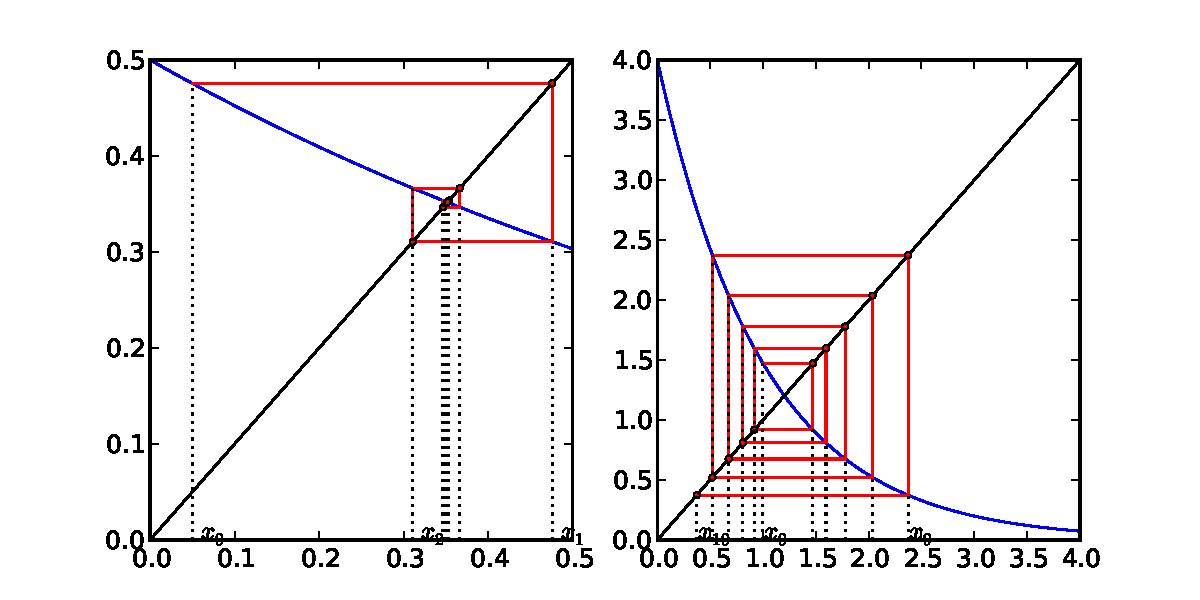
\includegraphics[width=\textwidth]{plots/banach}
  \caption{Sukzessive Substitution mit Funktion $g(r) = e^{-r}/\phi_0$
    mit $\phi_0=2$ (links) und $\phi_0=1/4$ (rechts). Blau
    durchgezogen ist die Funktion $g$, die Winkelhalbierende ist
    schwarz dargestellt. Die Punkte auf der Winkelhalbierenden
    markieren die Punkte $(x_1,x_1)$, $(x_2,x_2)$ usw., durch die das
    Lot auf $g$ gefällt wird, um den nächsten Punkt der sukzessiven
    Substitution zu erhalten. Im linken Graph sind die ersten sieben
    Glieder dargestellt, die exponentielle Konvergenz ist gut zu
    sehen. Im rechten Graph konvergiert das Verfahren nicht mehr.}
  \label{fig:banach}
\end{figure}

\subsection{Beispiel}

Als Beispiel für eine Anwendung des Banachschen Fixpunktsatzes
betrachten wir die dimensionslose Form des Yukawa- oder
Debye-Hückel-Potentials $\phi(r) = e^{-r}/r$. Wir fragen uns, wann für
welches $r$ dieses Potential einen gegeben Wert $\phi_0$ annimmt. Das
führt zu der Fixpunktgleichung
\begin{equation}
  g(r) = \frac{e^{-r}}{\phi_0} = r
\end{equation}
Die linke Seite ist eine auf $[0,\infty)$ L-stetige Funktion mit
$L=1/\phi_0$, wie man durch Ableiten leicht sieht.

Abbildung~\ref{fig:banach} zeigt die sukzessive Substitution für
$g(r)$. Graphisch lässt sich das Verfahren visualisieren, in dem in
jeder Iteration der Funktionswert $x_{n+1} = y =g(x_{n})$ an der
Winkelhalbierenden $y=x$ auf die $x$-Achse zurückgespiegelt wird. Im
linken Graph ist $\phi_0=2$ und damit $L=1/2$, so dass die sukzessive
Substitution exponentiell konvergiert. Für das letzte abgebildete
Glied, $x_7$, gilt $\abs{x_7-\overline{x}} \le 1/2^8 = 1/256$. Im
rechten Graph ist $\phi_0=1/4$ und damit $L=4$. Insbesondere ist auch
im Fixpunkt $g'(\overline(x))>1$. Abgebildet sind die ersten zehn
Glieder der sukzessiven Substitution, die hier nicht mehr
konvergiert. Wird hingegen $\phi_0$ so gewählt, dass 
$g'(\overline(x))<1$, aber $L>1$, so konvergiert das Verfahren zwar
noch, aber nicht mehr exponentiell.

\section{Newtonverfahren in einer Dimension}
\index{Newtonverfahren}
\index{Nullstellensuche}

Nachdem wir bis jetzt die suzessive Substitution zur Bestimmung von
Fixpunkten betrachten haben, geht es nun um die Nullstellensuche. Sei
also zunächst eine stetig differenzierbare Funktion $f:[a,b]\to\RR$
gegeben und deren Nullstellen $x$, $f(x) = 0$, gesucht. Ähnlich wie
bei der sukzessiven Iteration starten wir mit einem Startwert
$x_0$. Um uns nun der Nullstelle der Funktion zu nähern, linearisieren
wir in der aktuellen Näherung $x_n$ und lösen nach der Nullstelle
$x_{n+1}$ auf:
\begin{equation}
  x_{n+1} = g(x_n) := x_n - \frac{f(x_n)}{f'(x_n)}\quad\text{für}\; n\ge 0,
\end{equation}
wobei wir annehmen, dass $f'(x)\neq 0$ auf $[a,b]$.  Für eine
Nullstelle $\overline{x}$ von $f$ gilt offenbar $g(\overline{x}) =
\overline{x}$, d.h. wir suchen einen Fixpunkt von $g$.

Ist nun $f$ sogar zweifach stetig differenzierbar, so gilt
\begin{equation}
  g'(x) = 1 - \frac{f'(x)^2 - f(x)f''(x)}{f'(x)^2} =
  \frac{f(x)f''(x)}{f'(x)^2} \implies g'(\overline{x}) = 0.
\end{equation}
Das Newtonverfahren konvergiert also zumindest lokal gegen einen
Fixpunkt $\overline{x}$ von $g$ beziehungsweise eine Nullstelle von
$f$. Tatsächlich konvergiert das Verfahren wenigstens quadratisch,
wenn $f$ zweifach differenzierbar ist, da
\begin{align}
  x_{n+1} - \overline{x} = \frac{(x_n - \overline{x})f'(x_n) -
    f(x_n)}{f'(x_n)}
  = \frac{(x_n - \overline{x})}{f'(x_n)}\left( f'(x_n) -
    \frac{f(x_n) - f(\overline{x})}{x_n - \overline{x}}\right)\nonumber\\
  = \frac{(x_n - \overline{x})}{f'(x_n)}\left( f'(x_n) -
    f'(\xi')\right)
  = \frac{(x_n - \overline{x})^2}{}f''(\xi)
\end{align}
und somit
\begin{equation}
  \frac{\abs{x_{n+1} - \overline{x}}}{\abs{x_n - \overline{x}}^2}
  \le \frac{\max_{\xi\in [a,b]} \abs{f''(\xi)}}{\max_{\xi\in [a,b]} \abs{f'(\xi)}}
\end{equation}
Ist $f$ nur differenzierbar, so lässt sich ähnlich zeigen, dass das
Newtonverfahren superlinear konvergiert. Das Newtonverfahren
konvergiert also in jedem Fall schneller als die sukzessive
Substitution, erfordert allerdings eine mindestens stetig
differenzierbare Funktion.

\subsection{Beispiele}

\subsubsection{Wurzelziehen}

Wir betrachten die Gleichung $f(x) = x^k - a = 0$ auf der positiven
Halbachse. Dort konvergiert für jeden Startwert $x_0>0$ das
Newtonverfahren
\begin{equation}
  x_{n+1} = x_n - \frac{f(x_n)}{f'(x_n)} = \left(1 -
    \frac{1}{k}\right) x_n + \frac{1}{k} \frac{a}{x_n^{k-1}}
\end{equation}
gegen die einzige Nullstelle, nämlich die $k$-te Wurzel aus $a$. Für
$k=2$ ergibt sich das \emph{Heron-Verfahren} $x_{n+1} =
\frac{1}{2}\left(x_n + \frac{a}{x_n}\right)$, das bereits im 2. Jhdt. vor
Christus zum Wurzelziehen benutzt wurde.

\todo{Tabelle}

\subsubsection{Division}

Selbst die Division lässt sich als Newtonverfahren implementieren. Wir
betrachten also die Funktion $f(x) = \frac{1}{x} - a$, deren
Nullstelle wir suchen. Die Lösung kann mit Hilfe nur der
Grundrechenarten durch die Iteration
\begin{equation}
  x_{n+1} = x_n - \frac{f(x_n)}{f'(x_n)} = 2x_n - a x_n^2 
\end{equation}
bestimmt werden.

\subsection{Nullstellen von Polynomen}

Ist $p$ ein Polynom, so lassen sich dessen Nullstellen (approximativ)
mit Hilfe des Newtonverfahrens bestimmen:
\begin{equation}
  x_{n+1} = x_n - \frac{p(x_n)}{p'(x_n)},
\end{equation}
wobei $p(x_n)$ und $p'(x_n)$ durch ein modifiziertes Hornerschema
bestimmt werden können:
\begin{lstlisting}[language=C]
double newton_step(double *series, int n, double xn)
{
  double p = c[n];
  double dp = n*c[n];
  for(int i = n-1; i >= 0; --i) {
    p  =  p*xn +   c[i];
    dp = dp*xn + i*c[i];
  }
  return xn - p/dp;
}
\end{lstlisting}
Das Newtonverfahren liefert natürlich nur eine Nullstelle des
Polynoms. Durch die Polynomdivision, wieder mit Hilfe des
Hornerschemas wie in Abschnitt~\ref{sec:horner}, lässt sich diese
aber abspalten und das Newtonverfahren erneut starten, bis alle
Nullstellen gefunden sind.

\section{Regula falsi}

In vielen Fällen ist es nicht einfach oder unmöglich, die Ableitung
einer Funktion zu bestimmen. In diesem Fall kann man die Ableitung
durch die dividierte Differenz annähern, wobei nun zwei Startpunkte
$x_0$ und $x_1$ gebraucht werden. Daraus ergibt sich die \emph{Regula
  falsi}
\begin{equation}
  x_{n+1} = x_n - f(x_n)\frac{f(x_n) - f(x_{n-1})}{x_n - x_{n-1}},
\end{equation}
die nicht mehr quadratisch, aber wenigstens superlinear konvergiert.

Ein Beispiel, wo das Bestimmen der Ableitung unmöglich sind, sind
Computersimulationen im Druckgleichgewicht. Hier sucht man das jenige
Volumen, bei dem der mittlere Druck $P(V)$ dem vorgegebenen Außendruck
$P_0$ entspricht. Die Ableitung $dP(V)/dV$ ist in vielen Fällen nicht
zu bestimmen, da der mittlere Druck $P(V)$ ja Ergebnis einer Messung
in einer Simulation ist. In diesem Fall ist zusätzlich noch die
Funktion $P(V)$ mit einer oftmals nicht kleinen statistischen
Unsicherheit belegt. Trotzdem konvergiert die Regula falsi im
allgemeinen zufriedenstellend, solange keine zu hohen Ansprüche an die
Genauigkeit gestellt werden. Schliesslich kann die Nullstelle nicht
genauer als die vorhandenen Daten bestimmt werden.

\todo{Beispiel exp}

%\section{Bisektion}

%um Einzugrenzen

%\section{Newtonverfahren in mehreren Dimensionen}


%%% Local Variables: 
%%% mode: latex
%%% TeX-master: "padc"
%%% TeX-PDF-mode: t
%%% End: 
